% !TeX spellcheck = en_US
\chapter{Network Structures}
This chapter presents some common network structures and their capabilities.

\section{LeNet}
LeNet5 is probably the earliest \ac{CNN} network, proposed by \citeausm{lecun1998gradient}.

\begin{figure}[hbt!]
	\centering
	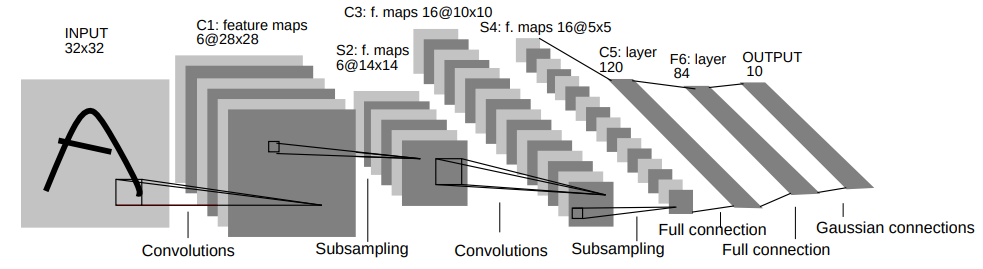
\includegraphics[width=\textwidth]{lenet.png}
	\caption{LeNet5 Architecture. \cite{lecun1998gradient}}
\end{figure}

Example coding with \texttt{pytorch} (\href{https://blog.paperspace.com/writing-lenet5-from-scratch-in-python/}{src}):
\begin{python}
import torch.nn as nn
	
class LeNet5(nn.Module):
	def __init__(self, num_classes):
		super(ConvNeuralNet, self).__init__()
		self.conv1 = nn.Sequential(
		nn.Conv2d(1, 6, kernel_size=5, stride=1, padding=0),
		nn.BatchNorm2d(6),
		nn.ReLU(),
		nn.MaxPool2d(kernel_size = 2, stride = 2))
		self.conv2 = nn.Sequential(
		nn.Conv2d(6, 16, kernel_size=5, stride=1, padding=0),
		nn.BatchNorm2d(16),
		nn.ReLU(),
		nn.MaxPool2d(kernel_size = 2, stride = 2))
		self.fc1 = nn.Sequential(
		nn.Linear(400, 120),
		nn.ReLU())
		self.fc2 = nn.Sequential(
		nn.Linear(120, 84),
		nn.ReLU())
		self.fc3 = nn.Linear(84, num_classes)
	
	def forward(self, x):
		...
		return y
\end{python}

\section{AlexNet}
The classic \ac{CNN} architecture for image classification on the CIFAR10 dataset \cite{krizhevsky2012imagenet}.

\begin{figure}[hbt!]
	\centering
	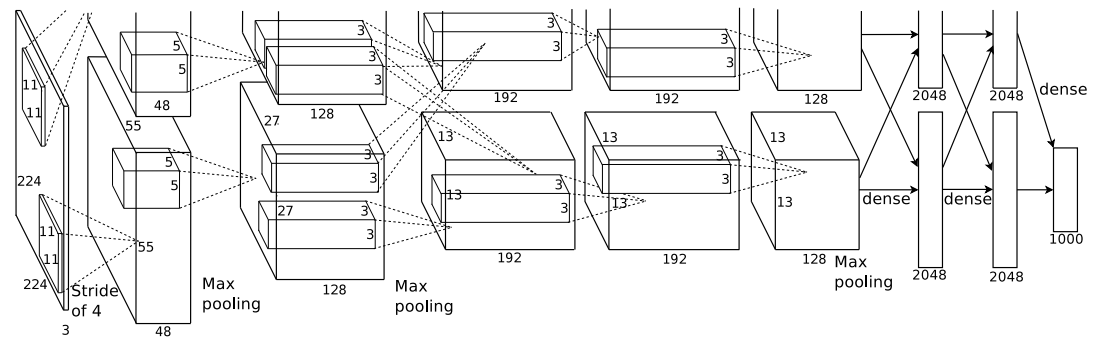
\includegraphics[width=\textwidth]{alexnet.png}
	\caption{AlexNet architecture. \cite{krizhevsky2012imagenet}}
\end{figure}

Example coding with \texttt{pytorch} (\href{https://blog.paperspace.com/alexnet-pytorch/}{src}):
\begin{python}	
class AlexNet(nn.Module):
	def __init__(self, num_classes=10):
		super(AlexNet, self).__init__()
		self.layer1 = nn.Sequential(
		nn.Conv2d(3, 96, kernel_size=11, stride=4, padding=0),
		nn.BatchNorm2d(96),
		nn.ReLU(),
		nn.MaxPool2d(kernel_size = 3, stride = 2))
		...
		self.fc1 = nn.Sequential(
		nn.Dropout(0.5),
		nn.Linear(4096, 4096),
		nn.ReLU())
		self.fc2= nn.Sequential(
		nn.Linear(4096, num_classes))
	
	def forward(self, x):
		...
		return y
\end{python}

\section{VGG Net}
The runner-up at the ILSVRC 2014 competition by \citeaus{simonyan2014very}:

\begin{figure}[hbt!]
	\centering
	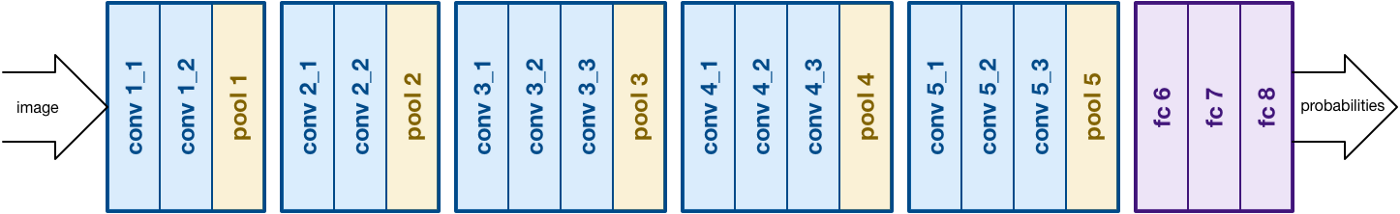
\includegraphics[width=\textwidth]{vggnet.png}
	\caption{The VGG Net architecture with 13 \ac{CONV} layers and 3 \ac{FC} layers. \cite{simonyan2014very}}
\end{figure}

Example coding with \texttt{pytorch} (\href{https://blog.paperspace.com/vgg-from-scratch-pytorch/}{src}):
\begin{python}
	class VGG16(nn.Module):
	def __init__(self, num_classes=10):
	super(VGG16, self).__init__()
	self.layer1 = nn.Sequential(
	nn.Conv2d(3, 64, kernel_size=3, stride=1, padding=1),
	nn.BatchNorm2d(64),
	nn.ReLU())
	...
	self.fc1 = nn.Sequential(
	nn.Dropout(0.5),
	nn.Linear(4096, 4096),
	nn.ReLU())
	self.fc2= nn.Sequential(
	nn.Linear(4096, num_classes))
	
	def forward(self, x):
	...
	return y
\end{python}

\section{Residual Network}
The \ac{ResNet} by \citeausm{he2016deep} tackles the vanishing gradient problem for deep neural network with the residual block (\figref{fig:residual-modul}). It creates a highway pass for the gradient to go to the early layers.
\begin{figure}[hbt!]
	\centering
	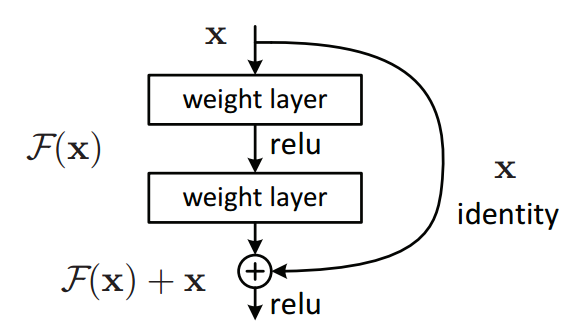
\includegraphics[width=0.5\textwidth]{residual-modul.png}
	\caption{Residual block \cite{he2016deep}.}
	\label{fig:residual-modul}
\end{figure}

Example coding with \texttt{pytorch} (\href{https://blog.paperspace.com/writing-resnet-from-scratch-in-pytorch/}{src}):
\begin{python}
class ResidualBlock(nn.Module):
	def __init__(self, in_channels, out_channels,
			stride = 1, downsample = None):
		super(ResidualBlock, self).__init__()
		self.conv1 = nn.Sequential(
		nn.Conv2d(in_channels, out_channels, kernel_size = 3,
		stride = stride, padding = 1),
		nn.BatchNorm2d(out_channels),
		nn.ReLU())
		self.conv2 = nn.Sequential(
		nn.Conv2d(out_channels, out_channels, kernel_size = 3,
		stride = 1, padding = 1),
		nn.BatchNorm2d(out_channels))
		self.downsample = downsample
		self.relu = nn.ReLU()
		self.out_channels = out_channels
	
	def forward(self, x):
		residual = x
		out = self.conv1(x)
		out = self.conv2(out)
		if self.downsample:
			residual = self.downsample(x)
		out += residual
		out = self.relu(out)
		return out
\end{python}

\begin{python}
class ResNet(nn.Module):
	def __init__(self, block, layers, num_classes = 10):
		super(ResNet, self).__init__()
		self.inplanes = 64
		self.conv1 = nn.Sequential(
		nn.Conv2d(3, 64, kernel_size = 7, stride = 2, padding = 3),
		nn.BatchNorm2d(64),
		nn.ReLU())
		self.maxpool = nn.MaxPool2d(kernel_size = 3, stride = 2, padding = 1)
		self.layer0 = self._make_layer(block, 64, layers[0], stride = 1)
		self.layer1 = self._make_layer(block, 128, layers[1], stride = 2)
		self.layer2 = self._make_layer(block, 256, layers[2], stride = 2)
		self.layer3 = self._make_layer(block, 512, layers[3], stride = 2)
		self.avgpool = nn.AvgPool2d(7, stride=1)
		self.fc = nn.Linear(512, num_classes)
		
	def _make_layer(self, block, planes, blocks, stride=1):
		downsample = None
		if stride != 1 or self.inplanes != planes:
			downsample = nn.Sequential(
				nn.Conv2d(self.inplanes, planes, kernel_size=1, stride=stride),
				nn.BatchNorm2d(planes),
				)
		layers = []
		layers.append(block(self.inplanes, planes, stride, downsample))
		self.inplanes = planes
		for i in range(1, blocks):
			layers.append(block(self.inplanes, planes))
		return nn.Sequential(*layers)
	
	def forward(self, x):
		x = self.conv1(x)
		x = self.maxpool(x)
		x = self.layer0(x)
		x = self.layer1(x)
		x = self.layer2(x)
		x = self.layer3(x)
		x = self.avgpool(x)
		x = x.view(x.size(0), -1)
		x = self.fc(x)
		return x
	
model = ResNet(ResidualBlock, [3, 4, 6, 3]).to(device)
\end{python}

\section{GoogLeNet}
\todo{}

\section{Comparison between Networks}
\begin{figure}[hbt!]
	\centering
	\begin{minipage}{.5\textwidth}
		\centering
		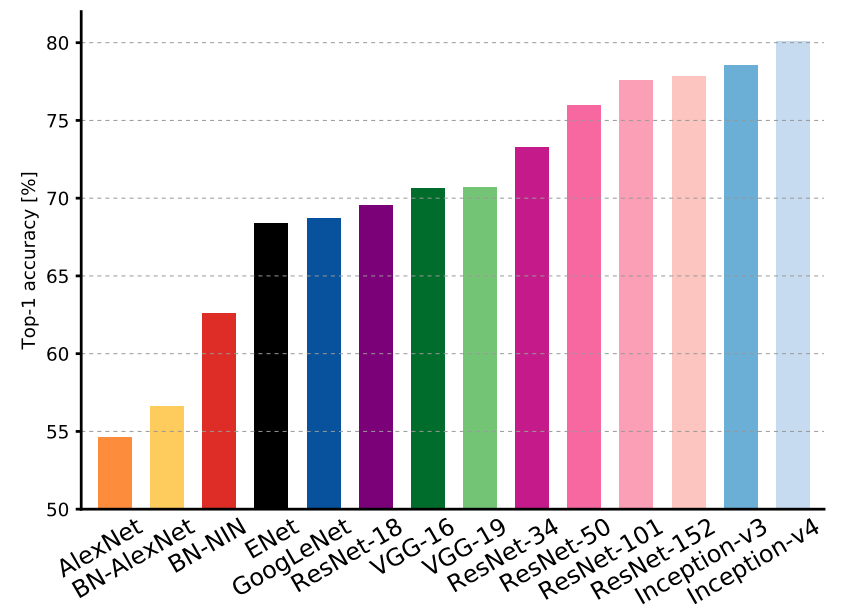
\includegraphics[width=0.95\textwidth]{top1accuracy-nets.png}
		\captionof{figure}{Top1 \ac{vs} network.}
		\label{fig:top1accuracy-nets}
	\end{minipage}%
	\begin{minipage}{.5\textwidth}
		\centering
		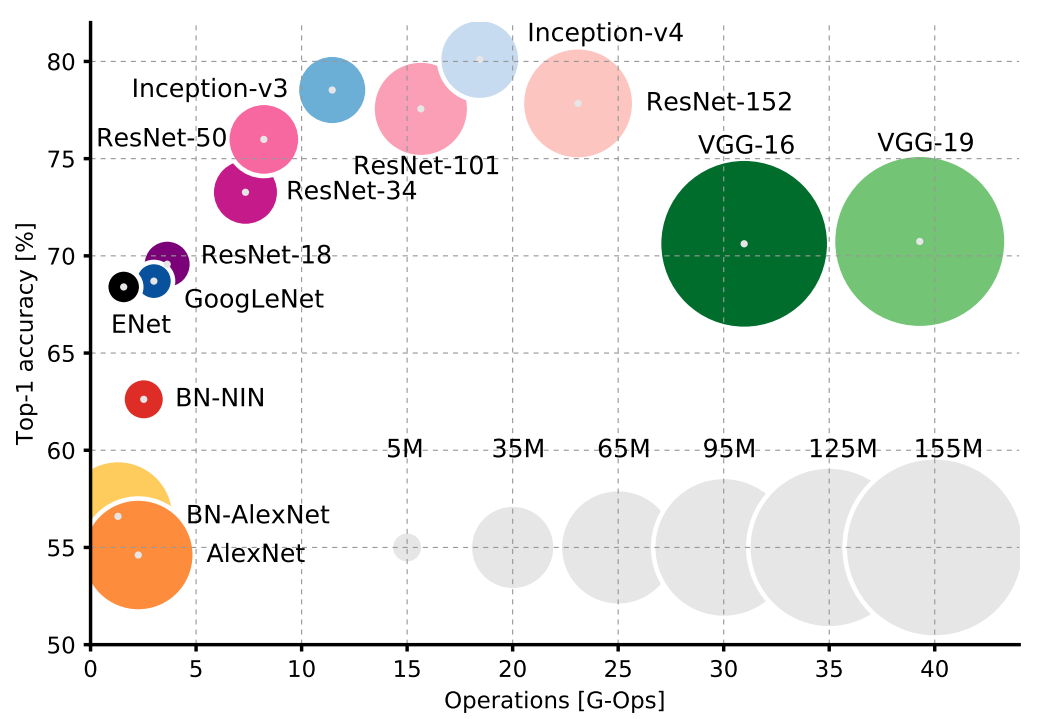
\includegraphics[width=0.95\textwidth]{top1accuracy-size-nets.png}
		\captionof{figure}{Top1 \ac{vs} operations, size $\propto$ \ac{param}.}
		\label{fig:top1accuracy-size-nets}
	\end{minipage}
\end{figure}

\section{Recurrent Neural Network}
The next three models deal with sequential data. It's a bit uncertain what is the original paper proposing the idea though \cite{elman1990finding}. \ac{BPTT}:\\
\todo{Add image, content}
\begin{align}
	\frac{\partial E_t}{\partial w_{ij}} &= \sum_{1 \leq k \leq t} \left( \frac{\partial E_t}{\partial h_t} \frac{\partial h_t}{\partial h_k} \frac{\partial h_k}{\partial w_{ij}} \right)\\
	E &= \sum_{1 \leq t \leq T} E_t\\
	\frac{\partial h_t}{\partial h_k} &= \prod_{t \geq i \geq k} \frac{\partial h_i}{\partial h_{i-1}}
\end{align}

\section{LSTM}
\cite{sutskever2014sequence} \todo{}

\section{Transformer}
\ac{RNN} suffers from vanishing/exploding gradient. \ac{LSTM} suffers from slow training time. \citeausm{vaswani2017attention} propose a approach based on the idea of attention. This approach can utilize the computation power of \ac{GPU} for parallelized matrix computation. This technique originally is meant for \ac{NLP} problem, but later on, also show meaningful application in \ac{CV}.

\begin{itemize}
	\item A easy and detailed explanation from \citeaus{alammar2020}
	This idea is the basis for GPT-3 \cite{brown2020language} and BERT \cite{devlin2018bert}
\end{itemize}
\begin{figure}[hbt!]
	\centering
	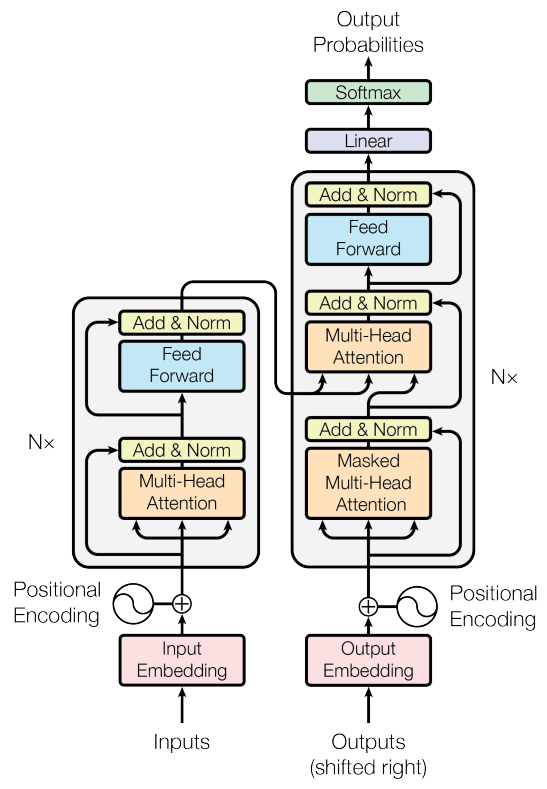
\includegraphics[width=0.5\textwidth]{transformer.png}
	\caption{The Transformer - model architecture \cite{vaswani2017attention}.}
\end{figure}

\begin{figure}[hbt!]
	\centering
	\begin{minipage}{.5\textwidth}
		\centering
		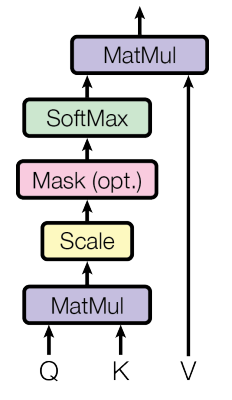
\includegraphics[width=0.55\textwidth]{transformer-1.png}
		\captionof{figure}{Scaled Dot-Product Attention.}
	\end{minipage}%
	\begin{minipage}{.45\textwidth}
		\centering
		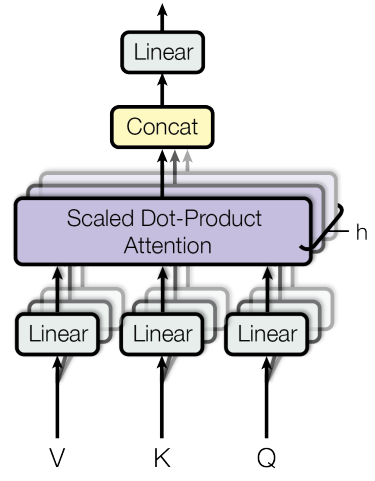
\includegraphics[width=0.82\textwidth]{transformer-2.png}
		\captionof{figure}{Multi-Head Attention.}
	\end{minipage}
\end{figure}

\section{U-Net}
The U-Net architecture by \citeaus{ronneberger2015u} can also be viewed as an encoder-decoder architecture \cite{kingma2013auto} with skip connections of \texttt{ResNet} (\figref{fig:unet1}). This structure is later adopted in \texttt{pix2pix} architecture for image-to-image translation \cite{isola2017image}.
\begin{figure}[hbt!]
	\centering
	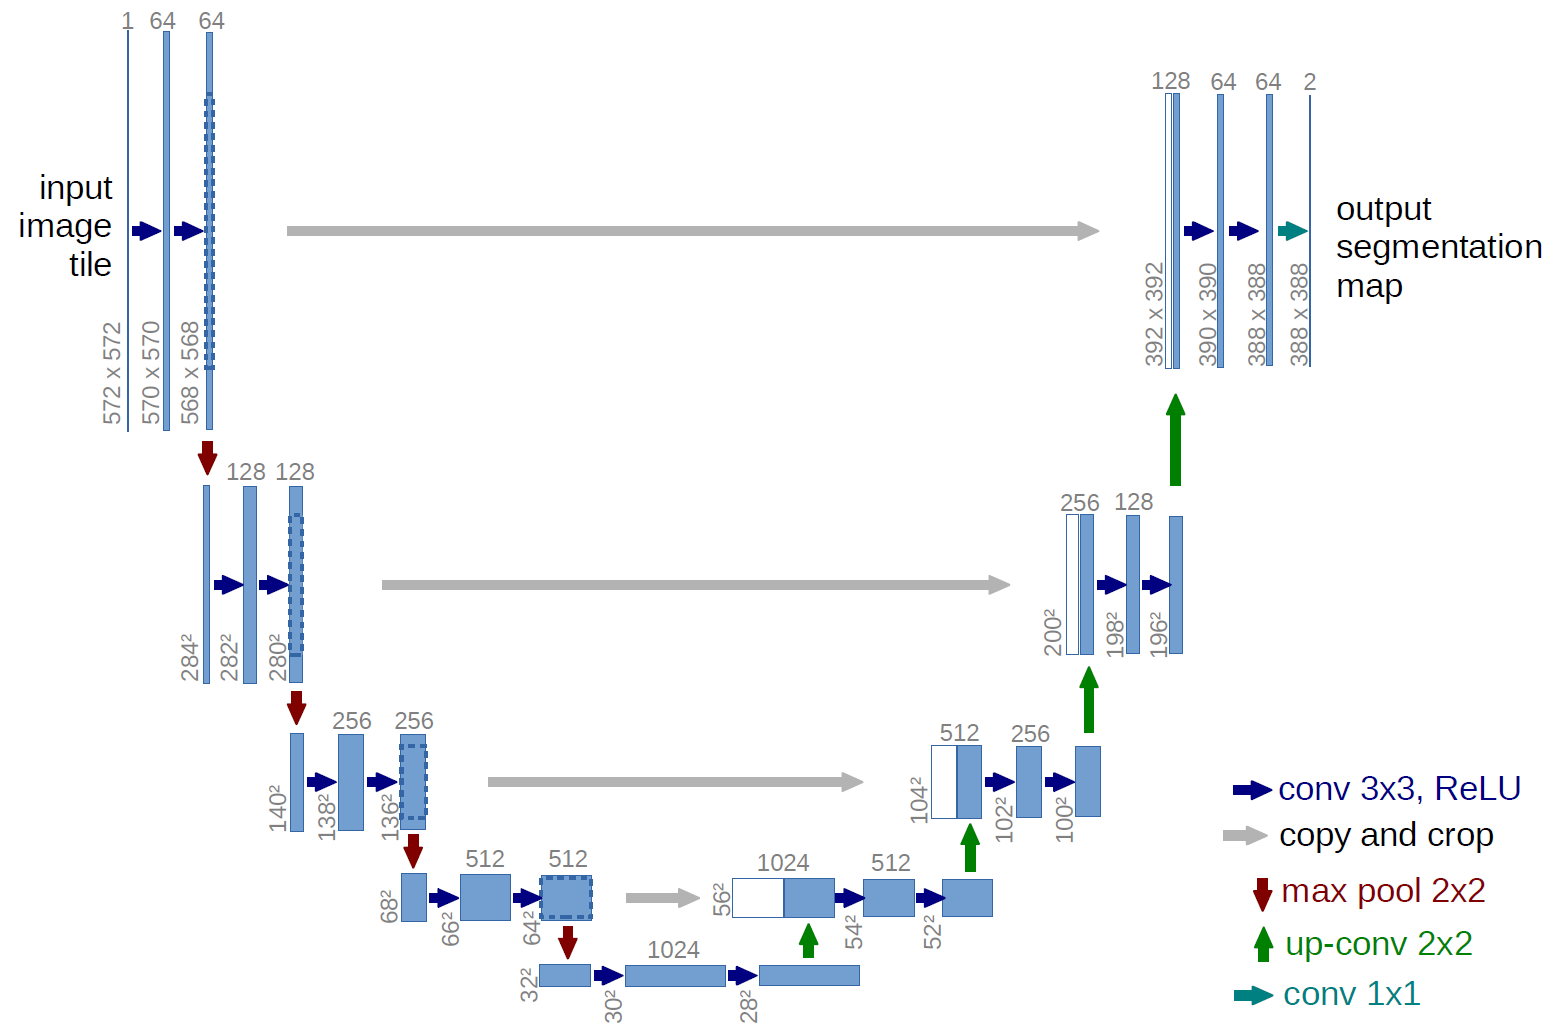
\includegraphics[width=0.9\textwidth]{unet.png}
	\caption{The U-Net architecture. \cite{ronneberger2015u}}
\end{figure}
\begin{figure}[hbt!]
	\centering
	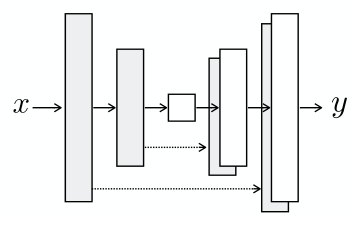
\includegraphics[width=0.35\textwidth]{unet1.png}
	\caption{The U-Net as a variational auto-encoder with skip connections. \cite{isola2017image}}
	\label{fig:unet1}
\end{figure}

\todo{benefits, comments?}

\section{Bayesian Neural Network}
Deep neural network's strength is its ability to approximate function. However, as powerful as it is, there is also a threat to overfit to the training data and fail to generalize on the test set. There are various techniques to reduce overfit and improve transfer learning, \eg, weight regularization, dropout, batch norm.

A conventional neural network takes in the same input and produce the same output. A Bayesian neural network different output when it takes in the same inputs twice. The resulting algorithm:
\begin{itemize}
	\item mitigates overfitting
	\item enables learning from small datasets
	\item tells us how uncertain our predictions are.
	\item adds stochasticity to neural network.
	\item Instead of weights, it has weights with distribution
	\begin{align}
		w_i \sim \mathcal{N}(\mu_i, \sigma_i^2)
	\end{align}
\end{itemize}

\note There is a thing called Bayesian Network, \ac{aka} belief network. That is not Bayesian neural network.

\begin{align*}
	\mathcal{D}_{tr} = \{\textbf{x}_i, y_i\}^n_{i=1}, \quad \text{model } F_\theta, \quad \text{loss } \mathcal{L}
\end{align*}
\begin{center}
	\begin{tabular}{p{7cm}|p{8cm}}
		Neural Network & Bayesian Neural Network\\ \hline \hline
		Training:
		\[\theta^* = \underset{\theta}{\arg\max} \sum_{(\textbf{x}_i, y_i)} \log [p(y_i | \textbf{x}_i, \theta)]\]
		\[\theta^* = \underset{\theta}{\arg\min} \sum_{(\textbf{x}_i, y_i)} \mathcal{L}(F_\theta(\textbf{x}_i), y_i)\] & Training:
		\[\mu^*, \Sigma^* = \underset{\mu, \Sigma}{\arg\max} \sum_{(\textbf{x}_i, y_i)} \log [p(y_i | \textbf{x}_i, \theta)] - KL[p(\theta), p(\theta_0)] \]
		\[\theta \sim \mathcal{N}(\mu, \Sigma), \qquad \theta_0 \sim \mathcal{N}(\textbf{0, I})\]
		\[\mu^*, \Sigma^* = \underset{\mu, \Sigma}{\arg\min} \sum_{(\textbf{x}_i, y_i)} \mathcal{L}(F_\theta(\textbf{x}_i), y_i) + KL[p(\theta), p(\theta_0)] \]
		\\ \hline
		Prediction:
		\[p(\hat{y} | \hat{\textbf{x}}, \theta^*)\]
		\[\hat{y} = F_{\theta^*}(\hat{\textbf{x}})\] & Prediction:
		\[p(\hat{y} | \hat{\textbf{x}}, \mathcal{D}_{tr}) = \int p(\hat{y} | \hat{\textbf{x}}, \theta^*) p(\theta^* | \mathcal{D}_{tr}) d\theta^* \]
		\[\theta^* \sim \mathcal{N}(\mu^*, \Sigma^*)\]
		\[\hat{y} = \frac{1}{K} \sum_{k=1}^K F_{\theta^*_k} (\hat{\textbf{x}}), \qquad \theta^*_k \sim \mathcal{N}(\mu^*, \Sigma^*)\]
	\end{tabular}
\end{center}

\subsection{Example}
\href{https://keras.io/examples/keras_recipes/bayesian_neural_networks/}{Keras's example}